\documentclass[11pt,twocolumn,twoside]{opticajnl}

\newcommand{\vect}[1]{\mathbf{#1}} % vector notation
\newcommand{\mat}[1]{\mathbf{#1}} % matrix notation
\renewcommand\Authands{, }

\usepackage{graphicx}
\graphicspath{ {./images/} }

\journal{opticajournal} % use for journal or Optica Open submissions

% See template introduction for guidance on setting shortarticle option
\setboolean{shortarticle}{true}
% true = letter/tutorial
% false = research/review article

% ONLY applicable for journal submission shortarticle types:
% When \setboolean{shortarticle}{true}
% then \setboolean{memo}{true} will print "Memorandum" on title page header
% Otherwise header will remain as "Letter"
\setboolean{memo}{false}

\title{Analysis of IRS double reflection effect on users' rate and corresponding sum-rate}


\author[1, *]{Alireza Tabatabaeian}
\author[1]{Danesh Abdollahi}
\author[1]{Mohammad Sadegh Jafari}
\author[1]{\\Mohammad Javad Emadi}

\affil[1]{Department of Electrical Engineering, Amirkabir University of Technology (Tehran Polytechnic), Tehran, Iran}
\affil[*]{alireza2541@aut.ac.ir}

\begin{abstract}
Abstract---This research explores the potential application of Intelligent Reflecting Surfaces (IRS) in the context of future communication networks, specifically focusing on 6G.
The study aims to optimize the weighted-sum-rate objective function for a realistic scenario involving two users.
In this scenario, the collaboration of two IRS units is considered, with a second-order reflection occurring between them.
One of the users experiences an obstacle, highlighting the need for improved network performance.
To enhance the communication network’s performance, a joint optimization approach is employed, optimizing both the passive beamforming coefficients of the IRS and the active beamforming coefficients of the antenna.
This optimization is carried out using a coordinate descent algorithm consisting of a gradient descent inside it, which iteratively refines the beamforming coefficients to maximize the overall system performance. 
The research also includes an evaluation of the Signal-to Interference-plus-Noise Ratio (SINR) improvement in the presence of the second-order reflection between the two IRS units.
The optimization process comprises several key steps.
Firstly, the Lagrangian dual transformation is applied to eliminate the logarithmic function, simplifying the optimization problem.
This transformation facilitates a more efficient and tractable optimization process.
Additionally, fractional programming techniques are employed to convert fractional terms into linear functions, further streamlining the optimization process.
These optimization techniques enable the exploration of optimal beamforming strategies and pave the way for enhanced performance in future wireless communication systems.
\newline \newline
Index Terms---IRS, Double Reflection, Sum-Rate, Coordinate Descent, Gradient Descent
\end{abstract}

\setboolean{displaycopyright}{false} % Do not include copyright or licensing information in submission.

\begin{document}

\maketitle

\section{Introduction}
The deployment of intelligent reflecting surfaces (IRS) in wireless communication systems has emerged as a promising technique to enhance the throughput and spectral efficiency. IRSs consist of a large number of reflective elements that can independently control the incident signals, enabling them to manipulate signal propagation. By strategically adjusting the phase shifts of these reflective elements, the IRS can shape the electromagnetic waves and achieve desired signal characteristics. This technology offers significant advantages, such as cost-effectiveness, low power consumption, and easy installation on various infrastructures. The integration of IRSs in 5G and 6G telecommunication wireless networks presents a new frontier in technology materials, revolutionizing the industry [1], [2]. These surfaces can be attached to walls or windows, reflecting unused portions of electromagnetic waves to increase special rates in wireless communication, such as sum-rate or secrecy-rate.
\par In [3], it provides an overview of IRS fundamentals including signal models, hardware architectures, and practical constraints. It also discusses key design aspects of IRS-aided wireless systems such as Reflection optimization, Channel estimation and Deployment strategy.
The [4] analyzes performance of IRS-aided communication between a single-antenna source and destination without a direct link, assisted by an IRS with M reflecting elements. Analytical expressions are derived for outage probability, symbol error rate, and achievable rate bounds. The analysis shows that the IRS can provide a diversity order equal to M. [5] proposes a scalable optimization framework for configuring large intelligent reflecting surfaces (IRSs) in wireless communication systems. IRSs can shape wireless propagation environments by introducing configurable signal reflections.
To enable scalable optimization, the IRS unit cells are partitioned into tiles. The response of each tile is modeled using concepts from physics and electromagnetics. This avoids optimizing each unit cell individually. A two-stage optimization approach is proposed - an offline design stage creates a codebook of transmission modes for each tile, and an online optimization stage selects the best transmission mode for each tile to optimize system performance.
For an example multi-user downlink communication system, algorithms are proposed to minimize transmit power while ensuring quality of service for each user by jointly optimizing the IRS configuration and the transmitter beamforming.
\par [6], the paper studies a wireless communication system where a transmitter (Alice) sends confidential messages to two receivers ($Bob_r$ and $Bob_t$) in the presence of two eavesdroppers ($Eve_r$ and $Eve_t$). A simultaneously transmitting and reflecting reconfigurable intelligent surface (STAR-RIS) is deployed to enhance security by improving the legitimate channel and energy harvesting at the eavesdroppers. The STAR-RIS can dynamically adjust its transmission and reflection coefficients (TARCs) to control signal propagation. The achievable secrecy rate and harvested energy are derived as functions of the TARCs.
\par Also in [7], the paper studies using reconfigurable intelligent surfaces (RISs) to assist free-space optical (FSO) communications for providing broadband internet access to high-speed trains (HSTs).
An RIS can control and redirect incident light beams through tuning its transmission/reflection coefficients. This can extend coverage and improve link reliability compared to direct FSO links from base stations. Analytical models are derived for the end-to-end channel statistics of direct and RIS-assisted FSO links under weak and moderate-to-strong atmospheric turbulence conditions. Performance is analyzed in terms of average SNR and outage probability for two RIS coverage scenarios: fixed-oriented reflection (FOR) where each RIS cell has a fixed coverage zone, and dynamic-oriented reflection (DOR) where the RIS dynamically tracks and reflects to the HST position.
\par [8], [9], [10], [11]  provide scenario for double reflection effect without considering the LoS effect.
[8] Proposes a double-IRS aided wireless communication system with two distributed IRSs deployed near the base station (BS) and user.
Assumes a rank-1 line-of-sight (LoS) channel between the two IRSs and optimizes the passive beamforming design to achieve a power gain scaling with $K^4$, where K is the total number of IRS elements.
Simulation results validate the $K^4$ power scaling achieved by deploying two cooperative IRSs with optimized passive beamforming, which outperforms the $K^2$ scaling of a single IRS system. [9] Studies channel estimation and passive beamforming design for a double-IRS aided single-user system. Proposes two channel estimation schemes: 1) estimates full channel matrix, 2) estimates two signature vectors for rank-1 LoS-dominant inter-IRS channel. Optimizes cooperative passive beamforming based on estimated channels to maximize achievable rate. Simulation results show significant rate enhancement of double-IRS system compared to single-IRS, especially with large number of elements.
[10] Considers a double-IRS system where signals reach the user via cascaded BS-IRS1-IRS2-user link only.
Optimizes transmit and passive beamforming using particle swarm optimization to maximize received signal power.
Results show excellent signal-to-noise ratio can be achieved despite no direct BS-user link, demonstrating feasibility of communication via double IRS reflection.
[11] Studies a double-IRS assisted multi-user MIMO system and proposes cooperative passive beamforming design. Analytically shows superior max SNR for single-user case and higher channel rank for multi-user case compared to single-IRS system. Proposes alternating optimization algorithm to maximize minimum SINR in multi-user case. Simulation results demonstrate significant rate gains of double-IRS system in various settings.
\par In summary, the four above papers study double-IRS assisted wireless communication systems under different system models and channel assumptions. The key focus is designing the cooperative passive beamforming over the two IRSs to achieve power scaling gains compared to single IRS systems. Both theoretical analysis and simulations demonstrate the performance gains of properly deployed double-IRS systems with optimized beamforming.

\par Notations: $x$ is scalar, $\vect{x}$ is vector, and $\mat{X}$ is matrix. Let $\mat{X}^T$, $\mat{X}^*$, and $\mat{X}^H$ denote the transpose, conjugate, and conjugate transpose of matrix $\mat{X}$, respectively. ${diag} (x_1, \ldots, x_n)$ represents a diagonal matrix with entries $x_1, \ldots, x_n$ on its main diagonal. $\mat{I}_M$ stands for $M \times M$ identity matrix. Operation ${Re}\{\mat{X}\}$ constructs a matrix by extracting the real parts of the entries of matrix $\mat{X}$, while operation $\angle(\mat{X})$ extracts the phases of elements of $\mat{X}$. The modulus of a complex number is denoted by $|\cdot|$, and $j = \sqrt{-1}$ is the imaginary unit. ${C}^{m \times n}$ represents the set of all $m \times n$ complex-valued matrices. Also the Hadamard product is denoted by $\odot$.
\par {\bf Organization}: The rest of this paper is organized as follows. 
In Section III, our proposed system model based on Double-Reflection-effect in IRS is introduced.
In Section IV, the sum-rate maximization problem subject to
power and unit modulus constraints is formulated.
In Section V, the proposed algorithm is described.
Numerical results are discussed in Section VI, and finally,
Section VII concludes the paper.

\section{Our Contribution}
At the moment, as you've seen, there are many papers and articles on the concept of intelligent reflecting surfaces. Not only a few of them considered the effect of double reflection or second-order reflection between IRS on the overall performance of the system, but also almost all of them neglect the effect of LoS in these scenarios applying an obstacle.
This neglecting was a motivation for us to propose a scenario to analyze the effect of double reflection in the presence of LoS signals. 
In this article, once and for all, we analyze the improvement achieved in the presence of double reflection to see that if it's rational to
neglect the double reflection effect or not.
\section{System Model}
- Without obstacle: In this scenario, both users have a direct line of sight to the antenna, and they also receive signals from both intelligent surfaces. Double reflection occurs between the intelligent surfaces. In this scenario, the weight of the users' reception rate is equal and set to a value of 1. Each user's receiver antenna has a single element, while the transmitting antenna has N elements. The intelligent surfaces, respectively, have $M_1$ and $M_2$ elements. In this scenario, each user receives signals from 5 different paths.

- With obstacle: In this scenario, only the second user has a direct line of sight to the antenna and receives signals from both intelligent surfaces. However, the first user does not have a direct line of sight to the transmitting antenna and only receives signals from first intelligent surface. Double reflection occurs between the intelligent surfaces. In this scenario, the weight of the users' reception rate is equal and set to a value of 1, but if needed, the weight of the first user can be increased due to receiving fewer signals. Each user's receiver antenna has a single element, while the transmitting antenna has N elements. The intelligent surfaces, respectively, have $M_1$ and $M_2$ elements. In this scenario, the first user receives signals from 2 paths, and the second user receives signals from 5 different paths, as depicted in the following diagram:

\begin{figure}[!h]
	\centering
	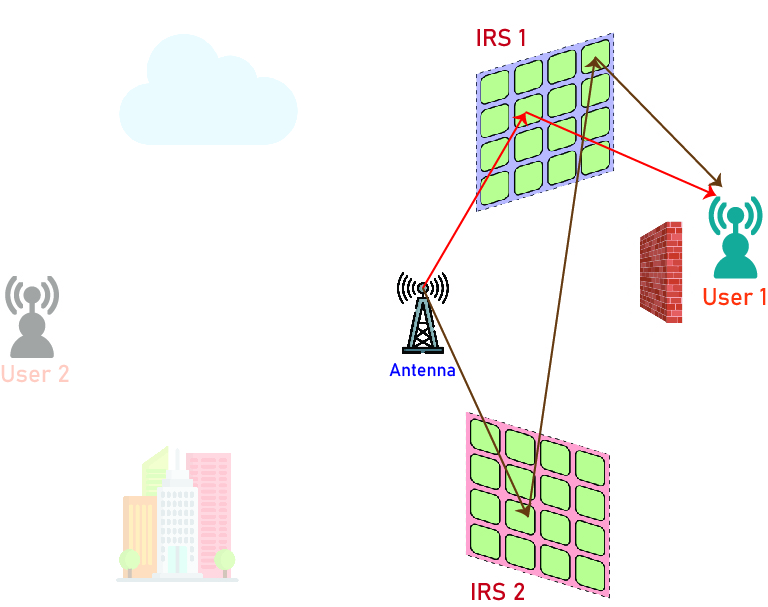
\includegraphics[scale=0.2]{with_obstacle__user1}
	
	\caption[User 1 system figure]{
		User 1 system figure
	}
\end{figure}

\begin{figure}[!h]
	\centering
	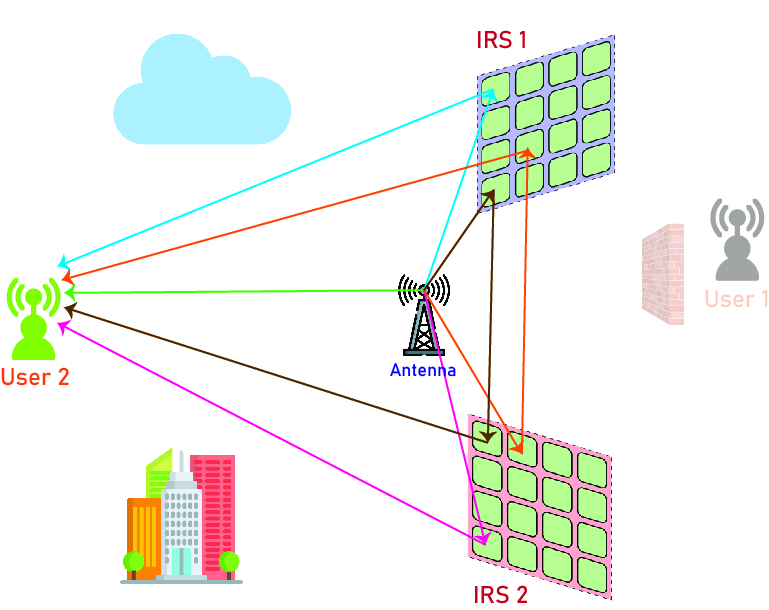
\includegraphics[scale=0.2]{with_obstacle__user2}
	
	\caption[User 2 system figure]{
		User 2 system figure
	}
\end{figure}

\subsection{Received Signal at \boldmath{$k$}-th user}
Denote the transmit data symbol to user $k$ by $s_k$. It is assumed that $s_k$ ($k = 1, \ldots, K$) are independent random variables with zero mean and unit variance. Then, the transmitted signal at the BS can be expressed as
\begin{equation}
	x = \sum_{k=1}^{K} w_k s_k, \label{eq:transmitted_signal}
\end{equation}
where $w_k \in \mathbb{C}^{N_t \times 1}$ is the corresponding transmit beamforming vector.

The received signal at user $k$ without considering the obstacles can be expressed as:
\begin{align*}
	y_k = &\underbrace{h_{d,k}^H x}_
	{\substack{\text{Direct link}}}
	+ \quad \\
	&\underbrace{h_{r_1,k}^H \Phi_1 G_1 x}_
	{\substack{\text{IRS1 link}}}
	+ \quad
	\underbrace{h_{r_2,k}^H \Phi_2 G_2 x}_
	{\substack{\text{IRS2 link}}}
	+ \quad \\ 
	&\underbrace{h_{r_1,k}^H \Phi_1 D \Phi_2 G_2 x}_
	{\substack{\text{Double reflection link}}}
	+ \quad
	\underbrace{h_{r_2,k}^H \Phi_2 D^H \Phi_1 G_1 x}_
	{\substack{\text{Double reflection link}}} +
	\underbrace{u_k}_
	{\substack{\text{AWGN}}}
\end{align*}

where $u_k \sim \mathcal{CN}(0, \sigma_0^2)$ denotes the additive white Gaussian noise (AWGN) at the $k$-th user receiver.

\subsection{SINR and Rate at \boldmath{$k$}-th user}
The $k$-th user treats all the signals from other users (i.e.,
$s_1$, ... , $s_{k-1}$, $s_{k+1}$, ... , $s_K$) as interference. Hence, the decoding SINR of $s_k$ at user $k$ is

\[
\gamma_k = \frac{{\left|\left(h_{d,k}^H + h_{r_1,k}^H \Phi_1 G_1 + h_{r_2,k}^H \Phi_2 G_2 + h_{r_1,k}^H \Phi_1 D \Phi_2 G_2 + h_{r_2,k}^H \Phi_2 D^H \Phi_1 G_1 \right)w_k\right|^2}}{{\sum_{i=1,i\neq k}^{K} \left|\left(h_{d,k}^H + h_{r_1,k}^H \Phi_1 G_1 + h_{r_2,k}^H \Phi_2 G_2 + h_{r_1,k}^H \Phi_1 D \Phi_2 G_2 + h_{r_2,k}^H \Phi_2 D^H \Phi_1 G_1 \right)w_i\right|^2 + \sigma^2_0}}
\]

\section{Problem Formulation}
aaaaaaaaaaaaaaaaaaaaaaaaaaaaaaaaaaaaaaaaaaaa
\subsection{Objective Function}
aaaaaaaaaaaaaaaaaaaaaaaaaaaaaaaaaaaaaaaaaaaa
\subsection{Constraints}
aaaaaaaaaaaaaaaaaaaaaaaaaaaaaaaaaaaaaaaaaaaa
\section{Proposed Algorithm}
aaaaaaaaaaaaaaaaaaaaaaaaaaaaaaaaaaaaaaaaaaaa
\subsection{Lagrangian Dual Transformation}
aaaaaaaaaaaaaaaaaaaaaaaaaaaaaaaaaaaaaaaaaaaa
\subsection{Multiple-ratio Fractional Programming}
aaaaaaaaaaaaaaaaaaaaaaaaaaaaaaaaaaaaaaaaaaaa
\subsection{Active Beamforming Optimization}

\subsection{Passive Beamforming Optimization}

\section{Numerical Results}

\subsection{Without Obstacle}

\subsection{With Obstacle}

\section{Conclusion}
Neglecting double reflection effect decreases the complexity of our problem because of the product term in system model.(change the sentence in a better way)

\begin{thebibliography}{1}
\bibitem{1}
M. D. Renzo, M. Debbah, D.-T. Phan-Huy, A. Zappone, M.-S.
Alouini, C. Yuen, V. Sciancalepore, G. C. Alexandropoulos, J. Hoydis,
H. Gacanin et al., “Smart radio environments empowered by reconfigurable AI meta-surfaces: An idea whose time has come,” EURASIP
Journal on Wireless Communications and Networking, vol. 2019, no. 1,
pp. 1–20, 2019.
\\
\bibitem{2}
Q. Wu and R. Zhang, “Towards smart and reconfigurable environment:
Intelligent reflecting surface aided wireless network,” IEEE Communications Magazine, vol. 58, no. 1, pp. 106–112, 2019.
\\
\bibitem{3}
Q. Wu, S. Zhang, B. Zheng, C. You and R. Zhang, "Intelligent Reflecting Surface-Aided Wireless Communications: A Tutorial," in IEEE Transactions on Communications, vol. 69, no. 5, pp. 3313-3351, May 2021, doi: 10.1109/TCOMM.2021.3051897.
\\
\bibitem{4}
D. Kudathanthirige, D. Gunasinghe and G. Amarasuriya, "Performance Analysis of Intelligent Reflective Surfaces for Wireless Communication," ICC 2020 - 2020 IEEE International Conference on Communications (ICC), Dublin, Ireland, 2020, pp. 1-6, doi: 10.1109/ICC40277.2020.9148760.
\\
\bibitem{5}
M. Najafi, V. Jamali, R. Schober and H. V. Poor, "Physics-based Modeling of Large Intelligent Reflecting Surfaces for Scalable Optimization," 2020 54th Asilomar Conference on Signals, Systems, and Computers, Pacific Grove, CA, USA, 2020, pp. 559-563, doi: 10.1109/IEEECONF51394.2020.9443337.
\\
\bibitem{6}
Kavianinia MR, Emadi MJ. Secrecy Rate Analysis of STAR-RIS in Presence of Energy Harvesting Eavesdroppers. arXiv preprint arXiv:2209.12105. 2022 Sep 24.
\\
\bibitem{7}
Agheli P, Beyranvand H, Emadi MJ. High-speed trains access connectivity through RIS-assisted FSO communications. Journal of Lightwave Technology. 2022 Aug 17;40(21):7084-94.
\\
\bibitem{8}
Han Y, Zhang S, Duan L, Zhang R. Cooperative double-IRS aided communication: Beamforming design and power scaling. IEEE Wireless Communications Letters. 2020 Apr 8;9(8):1206-10.
\\
\bibitem{9}
C. You, B. Zheng and R. Zhang, "Wireless Communication via Double IRS: Channel Estimation and Passive Beamforming Designs," in IEEE Wireless Communications Letters, vol. 10, no. 2, pp. 431-435, Feb. 2021, doi: 10.1109/LWC.2020.3034388.
\\
\bibitem{10}
Tian G, Song R. Cooperative beamforming for a double-IRS-assisted wireless communication system. EURASIP Journal on Advances in Signal Processing. 2021 Dec;2021:1-0.
\\
\bibitem{11}
B. Zheng, C. You and R. Zhang, "Double-IRS Assisted Multi-User MIMO: Cooperative Passive Beamforming Design," in IEEE Transactions on Wireless Communications, vol. 20, no. 7, pp. 4513-4526, July 2021, doi: 10.1109/TWC.2021.3059945.
\\
\bibitem{12}
K. Shen and W. Yu, "Fractional Programming for Communication Systems—Part I: Power Control and Beamforming," in IEEE Transactions on Signal Processing, vol. 66, no. 10, pp. 2616-2630, 15 May15, 2018, doi: 10.1109/TSP.2018.2812733.
\\
\bibitem{13}
Guo H, Liang YC, Chen J, Larsson EG. Weighted sum-rate maximization for intelligent reflecting surface enhanced wireless networks. In2019 IEEE Global Communications Conference (GLOBECOM) 2019 Dec 9 (pp. 1-6). IEEE.
\\
\bibitem{14}
Z. Li, M. Hua, Q. Wang and Q. Song, "Weighted Sum-Rate Maximization for Multi-IRS Aided Cooperative Transmission," in IEEE Wireless Communications Letters, vol. 9, no. 10, pp. 1620-1624, Oct. 2020, doi: 10.1109/LWC.2020.2999356.
\\
\bibitem{15}
Y. Ma, Y. Shen, X. Yu, J. Zhang, S. H. Song and K. B. Letaief, "A Low-Complexity Algorithmic Framework for Large-Scale IRS-Assisted Wireless Systems," 2020 IEEE Globecom Workshops (GC Wkshps, Taipei, Taiwan, 2020, pp. 1-6, doi: 10.1109/GCWkshps50303.2020.9367432.
\\
\end{thebibliography}

\end{document}
